\documentclass[a4paper,12pt]{article}

% =========================
% Подключение пакетов
% =========================
\usepackage[T2A]{fontenc}
\usepackage[utf8]{inputenc}
\usepackage[russian]{babel}

\usepackage{geometry}
\geometry{
    left=25mm,
    right=15mm,
    top=20mm,
    bottom=20mm
}

\usepackage{amsmath}
\usepackage{amssymb}
\usepackage{array}
\usepackage{booktabs}
\usepackage{float}
\usepackage{graphicx}
\usepackage{caption}
\usepackage{listings}
\usepackage{xcolor}
\usepackage{hyperref}

\hypersetup{
    colorlinks=true,
    linkcolor=black,
    urlcolor=blue
}

\lstdefinestyle{cppstyle}{
    language=C++,
    basicstyle=\ttfamily\small,
    keywordstyle=\color{blue},
    commentstyle=\color{gray},
    stringstyle=\color{red!60!black},
    numbers=left,
    numberstyle=\tiny,
    stepnumber=1,
    numbersep=8pt,
    tabsize=4,
    showstringspaces=false,
    breaklines=true,
    frame=single
}

\lstset{style=cppstyle}

% =========================
% Титульные данные
% =========================
\begin{document}

\begin{titlepage}
    \begin{center}

        \vspace*{5cm}

        {\Huge Московский Физико-Технический Институт}\\[2cm]

        {\LARGE Отчёт по эксперименту}\\[0.25cm]

        \noindent\rule{\textwidth}{1pt}
        \vspace*{-0.25cm}

        {\huge \textbf{Лабораторная по контейнерам}}

        \noindent\rule{\textwidth}{1pt}

        \vfill

    \end{center}

    \begin{flushright}
        \begin{minipage}{0.45\textwidth}
            {\Large
                Выполнил:\\
                Студент 1 курса ФАКТ\\
                Группа Б03-504\\
                Подмосковнов Лев
            }
        \end{minipage}
    \end{flushright}

    \vfill

    \begin{center}
        Долгопрудный\\2026
    \end{center}

\end{titlepage}
\restoregeometry

\setcounter{page}{2}

\newpage

% =========================
\section{Цель работы}

Цель лабораторной работы --- экспериментально исследовать время выполнения основных операций над контейнерами языка C++ и сравнить стандартные контейнеры STL с пользовательскими реализациями.

В работе рассматриваются следующие операции:
\begin{enumerate}
    \item добавление элемента в конец вектора;
    \item вставка элемента в произвольное место вектора;
    \item удаление элемента из произвольного места вектора;
    \item добавление элемента в начало односвязного списка;
    \item удаление элемента из начала односвязного списка;
    \item добавление элемента в бинарное дерево;
    \item обход всего контейнера.
\end{enumerate}

\section{Эксперимент 0. Добавление в конец вектора}

\subsection{Описание эксперимента}

В данном эксперименте исследуется изменение значений \texttt{size} и \texttt{capacity} контейнера \texttt{std::vector} при последовательном добавлении элементов с помощью \texttt{push\_back}.

\texttt{size} показывает фактическое количество элементов в векторе, а \texttt{capacity} --- количество элементов, которое может быть размещено в уже выделенной памяти без реаллокации.

\subsection{График}

На рисунке~\ref{fig:vector-capacity} должен быть представлен график зависимости \texttt{size} и \texttt{capacity} от номера итерации.

\begin{figure}[H]
    \centering
    
\includegraphics[width=0.85\textwidth]{t0/0.png}
    \caption{Изменение \texttt{size} и \texttt{capacity} при выполнении \texttt{push\_back}}
    \label{fig:vector-capacity}
\end{figure}

\subsection{Вывод}

Значение \texttt{size} увеличивается на единицу при каждом добавлении элемента. Значение \texttt{capacity} увеличивается скачками. Это связано с тем, что вектор заранее выделяет память с запасом, чтобы не выполнять реаллокацию при каждом вызове \texttt{push\_back}.

% =========================
\section{Эксперимент 1. Вставка элемента в произвольное место вектора}

\subsection{Описание эксперимента}

В этом эксперименте сравнивается среднее время вставки элемента в произвольное место для стандартного контейнера \texttt{std::vector} и пользовательского контейнера \texttt{subvector}.

Для стандартного вектора используется метод \texttt{insert}. Для пользовательского контейнера должна быть реализована аналогичная операция.

\subsection{Идея реализации}

Для вставки элемента в произвольную позицию необходимо:
\begin{enumerate}
    \item при необходимости увеличить ёмкость массива;
    \item сдвинуть все элементы справа от позиции вставки на одну ячейку вправо;
    \item записать новый элемент в освободившееся место;
    \item увеличить размер контейнера.
\end{enumerate}

\subsection{График}

\begin{figure}[H]
    \centering
    
\includegraphics[width=0.85\textwidth]{t1/1.png}
    % \fbox{\parbox{0.85\textwidth}{\centering Место для графика: среднее время insert для vector и subvector от size}}
    \caption{Среднее время вставки элемента в произвольное место вектора}
    \label{fig:vector-insert}
\end{figure}

\subsection{Асимптотика}

При вставке в произвольную позицию в среднем требуется сдвинуть порядка $\frac{n}{2}$ элементов. Поэтому средняя сложность операции:
\[
    T(n) = O(n).
\]

% =========================
\section{Эксперимент 2. Удаление элемента из произвольного места вектора}

\subsection{Описание эксперимента}

В данном эксперименте сравнивается среднее время удаления элемента из произвольного места для \texttt{std::vector} и пользовательского контейнера \texttt{subvector}.

Для стандартного контейнера используется метод \texttt{erase}. Для пользовательского контейнера должна быть реализована аналогичная операция.

\subsection{Идея реализации}

Для удаления элемента из произвольной позиции необходимо:
\begin{enumerate}
    \item выбрать позицию удаляемого элемента;
    \item сдвинуть все элементы справа от этой позиции на одну ячейку влево;
    \item уменьшить размер контейнера.
\end{enumerate}

\subsection{График}

\begin{figure}[H]
    \centering
    
\includegraphics[width=0.85\textwidth]{t2/2.png}
    % \fbox{\parbox{0.85\textwidth}{\centering Место для графика: среднее время erase для vector и subvector от size}}
    \caption{Среднее время удаления элемента из произвольного места вектора}
    \label{fig:vector-erase}
\end{figure}

\subsection{Асимптотика}

При удалении из произвольной позиции в среднем требуется сдвинуть порядка $\frac{n}{2}$ элементов. Поэтому средняя сложность операции:
\[
    T(n) = O(n).
\]

% =========================
\section{Эксперимент 3. Добавление элемента в начало односвязного списка}

\subsection{Описание эксперимента}

В данном эксперименте измеряется среднее время работы операции добавления элемента в начало списка для контейнеров:
\begin{itemize}
    \item \texttt{std::list};
    \item \texttt{std::forward\_list};
    \item пользовательского \texttt{subforward\_list}.
\end{itemize}

Для \texttt{std::list} и \texttt{std::forward\_list} используется метод \texttt{push\_front}. Для пользовательского контейнера используется метод \texttt{push\_forward}.

\subsection{График}

\begin{figure}[H]
    \centering
    
\includegraphics[width=0.85\textwidth]{t3/3.png}
    % \fbox{\parbox{0.85\textwidth}{\centering Место для графика: push\_front для list, forward\_list и subforward\_list от size}}
    \caption{Среднее время добавления элемента в начало списка}
    \label{fig:list-push-front}
\end{figure}

\subsection{Асимптотика}

Добавление в начало списка требует только создания нового узла и изменения указателя на начало списка. Поэтому сложность операции:
\[
    T(n) = O(1).
\]

% =========================
\section{Эксперимент 4. Удаление элемента из начала односвязного списка}

\subsection{Описание эксперимента}

В данном эксперименте измеряется среднее время удаления элемента из начала списка для контейнеров:
\begin{itemize}
    \item \texttt{std::list};
    \item \texttt{std::forward\_list};
    \item пользовательского \texttt{subforward\_list}.
\end{itemize}

Для стандартных контейнеров используется метод \texttt{pop\_front}. Для пользовательского контейнера используется метод \texttt{pop\_forward}.

\subsection{График}

\begin{figure}[H]
    \centering
    
\includegraphics[width=0.85\textwidth]{t4/4.png}
    % \fbox{\parbox{0.85\textwidth}{\centering Место для графика: pop\_front для list, forward\_list и subforward\_list от size}}
    \caption{Среднее время удаления элемента из начала списка}
    \label{fig:list-pop-front}
\end{figure}

\subsection{Асимптотика}

Удаление из начала списка требует изменения указателя на первый элемент и освобождения памяти удаляемого узла. Размер списка не влияет на количество выполняемых действий:
\[
    T(n) = O(1).
\]

% =========================
\section{Эксперимент 5. Добавление элемента в бинарное дерево}

\subsection{Описание эксперимента}

В этом эксперименте измеряется среднее время вставки элемента в ассоциативные контейнеры:
\begin{itemize}
    \item \texttt{std::set};
    \item \texttt{std::map};
    \item \texttt{std::multiset};
    \item \texttt{std::multimap}.
\end{itemize}

\subsection{График}

\begin{figure}[H]
    \centering
    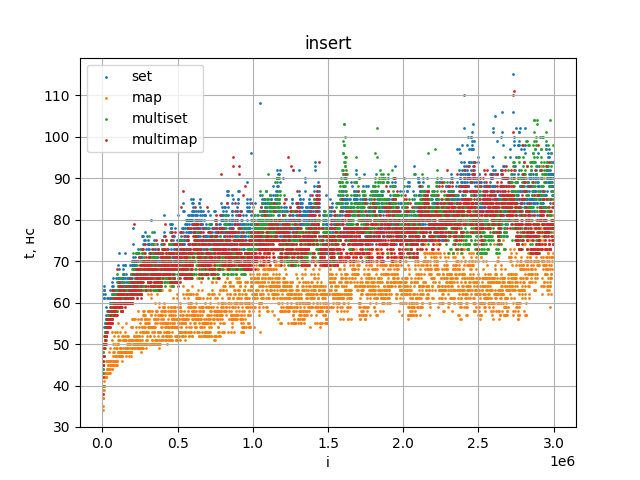
\includegraphics[width=0.85\textwidth]{t5/5.png}
    % \fbox{\parbox{0.85\textwidth}{\centering Место для графика: insert для set, map, multiset и multimap от size}}
    \caption{Среднее время вставки элемента в бинарное дерево}
    \label{fig:tree-insert}
\end{figure}

\subsection{Асимптотика}

Стандартные ассоциативные контейнеры STL обычно реализуются как сбалансированные деревья поиска. Высота такого дерева имеет порядок $\log n$, поэтому вставка элемента выполняется за:
\[
    T(n) = O(\log n).
\]

% =========================
\section{Эксперимент 6. Обход всего контейнера}

\subsection{Описание эксперимента}

В данном эксперименте измеряется среднее время полного обхода контейнеров:
\begin{itemize}
    \item \texttt{std::vector};
    \item \texttt{std::forward\_list};
    \item \texttt{std::list};
    \item \texttt{std::map};
    \item \texttt{std::set}.
\end{itemize}

В качестве простой операции за $O(1)$ используется арифметическая операция над каждым элементом. Для контейнеров, элементы которых можно изменять, можно увеличивать каждый элемент на единицу. Для \texttt{std::set} изменять элементы напрямую нельзя, поэтому для него можно использовать подсчёт контрольной суммы.

\subsection{График}

\begin{figure}[H]
    \centering
    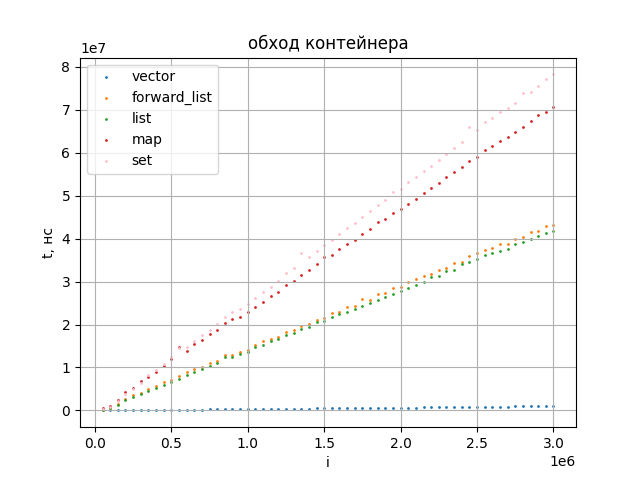
\includegraphics[width=0.85\textwidth]{t6/6.png}
    %\fbox{\parbox{0.85\textwidth}{\centering Место для графика: среднее время обхода vector, forward\_list, list, map, set от size}}
    \caption{Среднее время обхода всего контейнера}
    \label{fig:traverse}
\end{figure}

\subsection{Асимптотика}

При полном обходе необходимо посетить каждый элемент контейнера. Если обработка одного элемента занимает $O(1)$, то общая сложность:
\[
    T(n) = O(n).
\]

% =========================
\section{Сводная таблица асимптотик}

\begin{table}[H]
    \centering
    \caption{Теоретические асимптотики исследуемых операций}
    \label{tab:complexity}
    \begin{tabular}{>{\raggedright\arraybackslash}p{8cm} >{\centering\arraybackslash}p{4cm}}
        \toprule
        Операция                                                                             & Асимптотика \\
        \midrule
        \texttt{vector::push\_back} амортизированно                                          & $O(1)$      \\
        \texttt{vector::push\_back} при реаллокации                                          & $O(n)$      \\
        Вставка в произвольное место \texttt{vector} / \texttt{subvector}                    & $O(n)$      \\
        Удаление из произвольного места \texttt{vector} / \texttt{subvector}                 & $O(n)$      \\
        Добавление в начало \texttt{list}, \texttt{forward\_list}, \texttt{subforward\_list} & $O(1)$      \\
        Удаление из начала \texttt{list}, \texttt{forward\_list}, \texttt{subforward\_list}  & $O(1)$      \\
        Вставка в \texttt{set}, \texttt{map}, \texttt{multiset}, \texttt{multimap}           & $O(\log n)$ \\
        Полный обход контейнера                                                              & $O(n)$      \\
        \bottomrule
    \end{tabular}
\end{table}

% =========================
\section{Общий вывод}

В ходе лабораторной работы были исследованы временные характеристики основных операций над стандартными и пользовательскими контейнерами C++.

Эксперимент с \texttt{std::vector} показал, что его размер увеличивается линейно, а ёмкость --- скачкообразно. Это подтверждает механизм резервирования памяти с запасом. Операция \texttt{push\_back} имеет амортизированную сложность $O(1)$, но отдельные операции реаллокации могут выполняться за $O(n)$.

Вставка и удаление элемента из произвольного места вектора имеют линейную сложность $O(n)$, так как требуют сдвига элементов. Пользовательский контейнер \texttt{subvector} должен демонстрировать аналогичную асимптотику при корректной реализации.

Добавление и удаление элемента из начала списков выполняется за $O(1)$, так как для этого достаточно изменить один или несколько указателей. Поэтому графики для \texttt{std::list}, \texttt{std::forward\_list} и \texttt{subforward\_list} должны быть близки к горизонтальным.

Вставка в ассоциативные контейнеры \texttt{std::set}, \texttt{std::map}, \texttt{std::multiset} и \texttt{std::multimap} выполняется за $O(\log n)$, поскольку эти контейнеры основаны на сбалансированных деревьях поиска.

Полный обход любого контейнера требует посещения каждого элемента, поэтому имеет сложность $O(n)$. При этом фактическое время обхода может отличаться из-за особенностей хранения данных в памяти: \texttt{std::vector} хранит элементы непрерывно, а списки и деревья используют отдельные узлы, расположенные в разных участках памяти.

% =========================
\end{document}
